%-*-coding: utf-8-*-

\chapter{Обзор предметной области}

\section{Вспомогательные понятия}

\subsection{Векторное представление слов}
Векторное представление слова (word embedding)\cite{Bengio03aneural}~--- параметризованное отображение слова на пространство большой размерности $\mathbb{R}^d$. 
Такое представление сохраняет семантические отношения между словами. 
Причем, похожим словам сопоставляются близкие по некоторой метрике вектора, 
а различным~--- удаленные друг от друга.

Векторное представление слов либо обучают <<с нуля>> вместе с основной моделью, либо берут за основу предобученные на достаточно большом корпусе текстовых данных. Наиболее крупные корпусы векторных представлений это word2vec\cite{DBLP:journals/corr/MikolovLS13, wor2vec}, а также GloVe\cite{pennington2014glove, glove}, которые также будут использоваться в данной работе.

\subsection{Дерево синтаксического разбора предложения}
Существует несколько способов построения дерева синтасксического разбора.
Это зависит от принципов построения и сущностей, которые поддерживает дерево зависимостей.
Так, например, существуют Stanford Dependencies\cite{standeps}, а также Universal Dependencies\cite{unideps}.
В данной работе будет использоваться преимущественно способ Probabilistic Context-Free Grammars\cite{pcfg}.

Данный способ задается грамматикой, по которой и разбирается предложение\cite{Klein03accurateunlexicalized}.
По языку строятся подкатегории фраз, например, такие как "noun phrase" (NP), "verb phrase" (VP) и т.д. 
Для них также строятся правила вывода грамматики. После чего предложение разбирается по этим правилам. 

\begin{figure}[h]
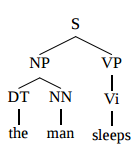
\includegraphics[scale=0.9]{pcfgs}
\caption{\textbf{Пример разбора предложения PCFG парсером}}
\label{fig:pcfgs}
\end{figure}

Данная граматика может быть неоднозначна, 
поэтому вывод происходит вероятностно~--- выбирается наиболее вероятное правило в данном контексте.

Вообще говоря, предложенная модель не зависит от способа построения дерева разбора и языка.

\section{Постановка задачи}
\noindent Пусть есть некоторый язык со словарем $V$.\\
Пусть есть некоторая функция ошибки $L:\mathbb{R}^s \to \mathbb{R}$.\\
Пусть $D$~--- множество последовательностей над $V$, называемое датасетом задачи.\\
Задача построения векторного представления предложения, состоит в изобретении такой модели $M$, 
которая для любой последовательности слов $w \in V^n$ (любому предложению) сопоставляет
вектор $M(w) \in \mathbb{R}^s$ так, что суммарная ошибка $$\sum_{w \in D} L(M(w))$$ была как можно меньше.
Чем меньше эта ошибка, тем более качественна модель $M$.\\

\section{Обзор существующих решений}

В данной главе будут приведены существующие решения для построения векторного представления предложения.

\subsection{Paragraph Vector}
Целью подхода Paragraph Vector является сопоставление вещественного вектора в $\mathbb{R}^d$ последовательности слов произвольной длины: предложению, абзацу или даже документу\cite{DBLP:journals/corr/LeM14}.
Paragraph Vector учитывает семантический контекст текста на котором он получен.

Параметрами Paragraph Vector являются: вещественная матрица $W$~--- векторное представление слов словаря текстового корпуса, а также вещественная матрица $D$~--- векторное представление абзацев корпуса. Метод пытается предсказать следующее слово в абзаце, опираясь на векторное представление данного абзаца, а также слов из абзаца, смежных с предсказываемым словом, то есть находящихся в одном контексте с ним.
Данный метод может быть также применен к предложению.

\begin{figure}[h]
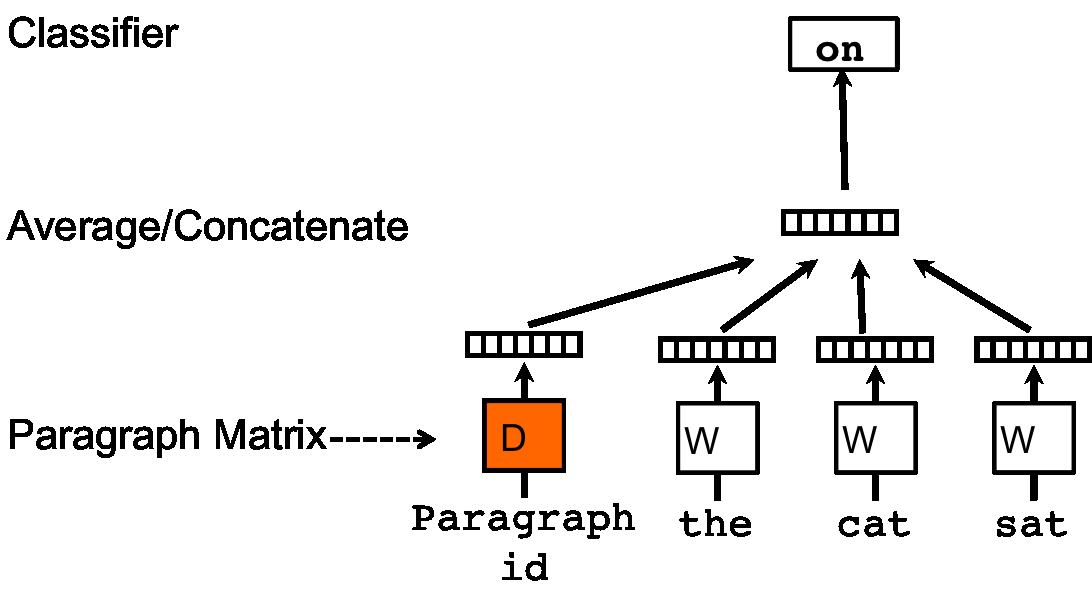
\includegraphics[scale=0.65]{par_vec}
\caption{\textbf{Paragraph Vector}}
\label{fig:par_vec}
\end{figure}

\subsection{Рекуррентная нейронная сеть} \label{lstm}
Основным инструментом для обработки текстов являются так называемые \emph{рекуррентные нейронные сети}(РНС)\cite{Goller96learningtask-dependent}.

Рекуррентные нейронные сети предназначены (РНС) для обработки последовательных данных, таких как звук и текст. В традиционных нейронных сетях все входы считаются независимыми друг от друга, но для многих задач это не так, и такой подход не учитывает много информации о структуре данных.

РНС принимает слова последовательности поочереди, сохраняя внутри себя контекст уже принятого текста. Рекуррентными они называются потому что выполняют одну и ту же задачу для каждого слова в тексте. Данная архитекутра достаточно хорошо отражает процесс восприятия информации человеком: после того как мы прочли начало предложение, в нашей голове уже сформировался некоторый контекст, и следующее слово обрабатывается нами с учетом уже прочитанной информации, а не воспринимается с чистого листа.

\begin{figure}[h]
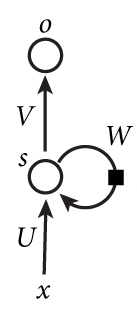
\includegraphics[scale=0.7]{rnn}
\caption{\textbf{РНС}}
\label{fig:rnn}
\end{figure}

\begin{figure}[h]
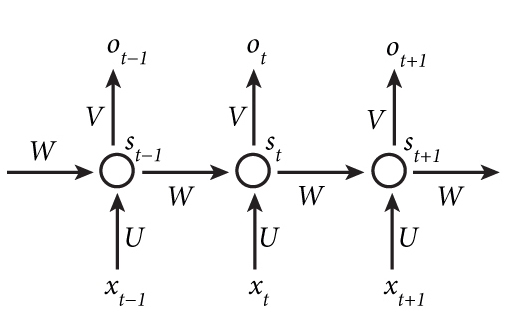
\includegraphics[scale=0.7]{rnn-unfold}
\caption{\textbf{РНС в развернутом виде}}
\label{fig:rnn-unfold}
\end{figure}

\noindent $U, W, V$~--- параметры РНС сети\\
$x_t$~--- вектор, соответствующий слову $t$ \\
$s_t$~--- информация о первых $t$ словах \\
$o_t$~--- выходной вектор

Хотя РНС является достаточно мощной моделью, у нее есть ряд недостатков, самый большой из которых~--- это так называемая <<проблема затухания градиента>>. Суть ее заключается в том, что РНС не может запоминать контекст начала предложения в длинных последовательностях слов. Поэтому на смену РНС была изобретена другая архитектура РНС, под названием \emph{долгая краткосрочная память} (ДКП) (от англ. Long Short Term Memory или LSTM), которая решает эту проблем\cite{Hochreiter:1997:LSM:265493.264179}. Одна ячейка ДКП:
$$i_t=\sigma \left( W^{(i)}x_t+U^{(i)}h_{t-1} + b^{(i)} \right)$$
$$f_t=\sigma \left( W^{(f)}x_t+U^{(f)}h_{t-1} + b^{(f)} \right)$$
$$o_t=\sigma \left( W^{(o)}x_t+U^{(o)}h_{t-1} + b^{(o)} \right)$$
$$u_t=\tanh \left( W^{(u)}x_t+U^{(u)}h_{t-1} + b^{(u)} \right)$$
$$c_t=i_t \odot u_t + f_t \odot c_{t-1}$$
$$h_t=o_t \odot tanh(c_t)$$
где $W^{(i)}, W^{(f)}, W^{(o)}, W^{(u)} \in \mathbb{R}^{a \times h},\\U^{(i)}, U^{(f)}, U^{(o)}, U^{(u)} \in \mathbb{R}^{h \times h},\\b^{(i)}, b^{(f)}, b^{(o)}, b^{(u)} \in \mathbb{R}^{h}$~--- параметры модели\\
$x_t \mathbb{R}^a$~--- one-hot вектор $t$-го слова предложения

Таким образом, на вход ДКП подается предложение и в качестве векторного представления используется
последний вектор $h_n$.

\subsection{Сверточная нейронная сеть}
Сверточная нейронная сеть (СНС)~--- успешно показала себя в обработке и анализе изображений. Они работают подобно тому, как происходит распознавание образов в головной коре человека. СНС состоят из нескольких слоев, каждый из которых детектирует некоторые визуальные признаки изображения, такие как прямые линии, окружности. Признаки с предыдущего слоя используются для формирования более высокоуровневых визуальных признаков.

Преимуществом СНС является выделение локалных пространственных признаков. В контексте изображений это означает, что визуальные признаки локализуются сначала на неболших квадратах, а далее объединяются в большие фигуры.

Оказывается, данный плюс можно использовать и для построения векторного представления, 
если рассмотреть слова предложения как вектора некоторой размерности. Тогда если в предложении $n$ слов, 
и размерность векторного представления слова $d$, получаем матрицу $n \times d$, 
которую можно трактовать как изображение и применить к нему сверточную нейронную сеть\cite{Lecun98gradient-basedlearning, DBLP:journals/corr/Kim14f}.

\begin{figure}[h]
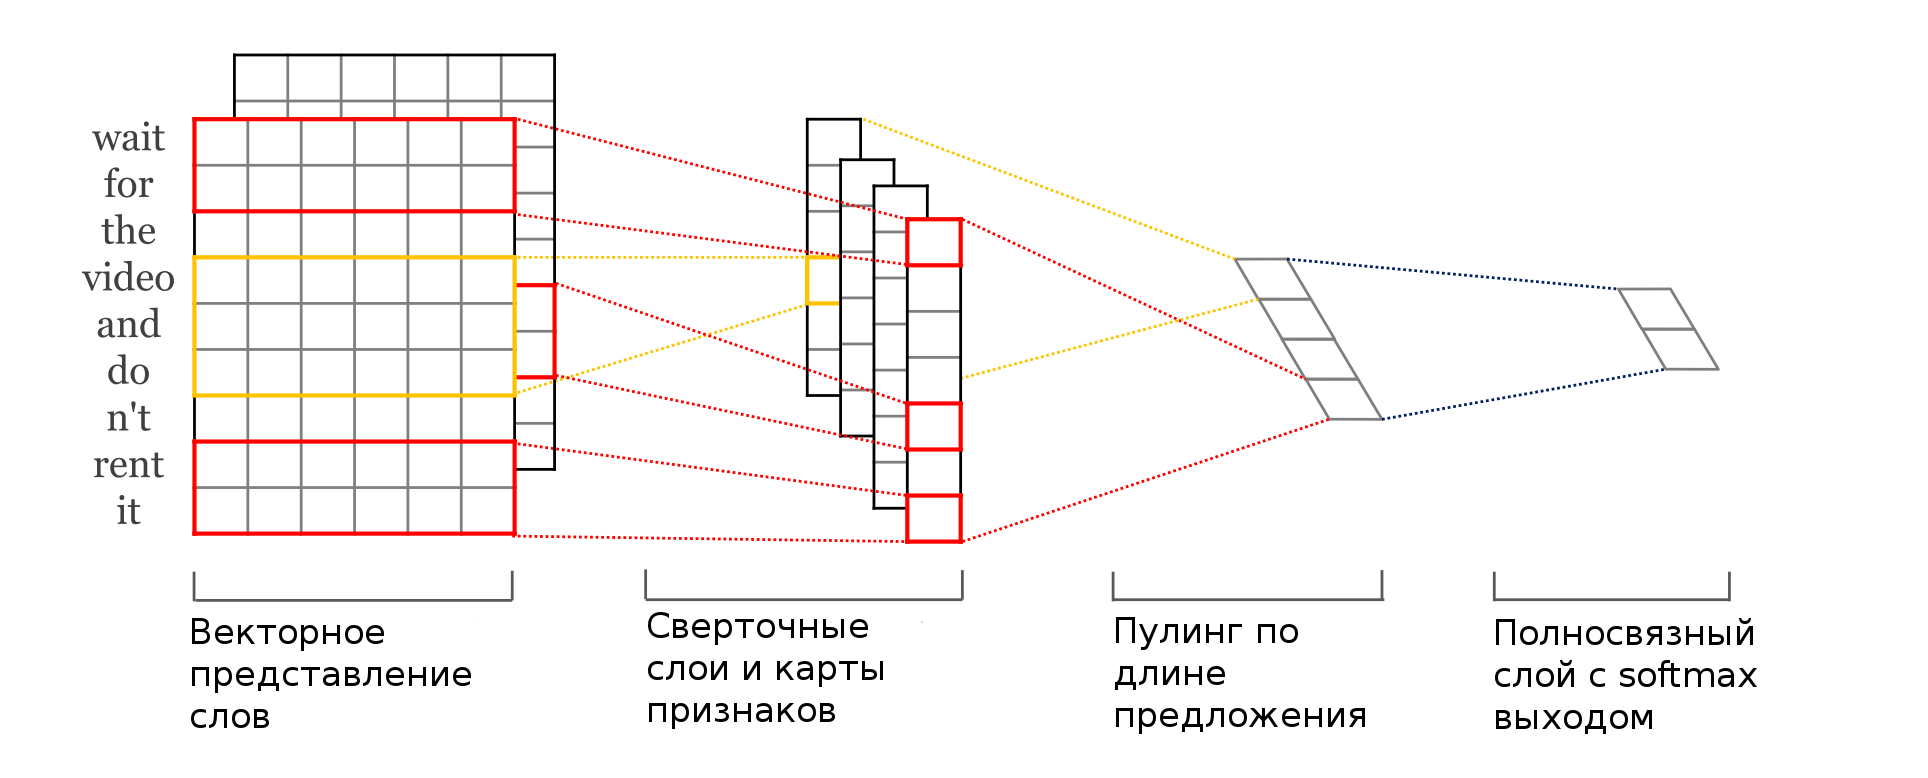
\includegraphics[scale=0.55]{cnn-rus}
\caption{\textbf{СНС для предложения}}
\label{fig:cnn}
\end{figure}

\subsection{Рекуррентная тензорная нейронная сеть}
Еще одним важным подходом для построения векторного представления является использование 
дерева синтаксического разбора предложения. Вообще говоря, решения, использующие этот подход, предполагают, что у предложения уже построено дерево синтаксического разбора. Построение дерева является отдельной достаточно важной задачей NLP. На данный момент существуют алгоритмы, которые делают это построение с очень хорошей точностью\cite{lex-parser, chen2014fast}. 
С другой стороны, обычно для таких решений не столь важно точное построение дерева, то есть они не критичны к неточностям в дереве разбора.

Рекуррентная тензорная нейронная сеть (РТНС)~--- одно из решений, использующее дерево синтаксического разбора. Целью данного метода является сопоставление каждой вершине дерева разбора вектора в $\mathbb{R}^d$, 
который и характеризует семантическое содержание фразы, соответствующей поддереву этой вершины.
Вектор для вершины $p$ вычисляется как $f(p)=g(f(c_1), f(c_2) \dots{} f(c_k))$, где $c_i$~--- непосредственные потомки вершины $p$, а $g$~--- некоторая функция. Вычисление происходит снизу-вверх, то
есть от листьев дерева к его корню. Для листьев $f(p)$ берутся произвольными и улучшаются в результате обучения в соответствии с поставленной задачей.
В качестве функции $g$ в оригинальной работе\cite{socher-EtAl:2013:EMNLP} используется умножение на $n$-мерный тензор.

\begin{figure}[h]
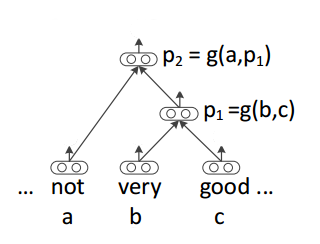
\includegraphics[scale=0.7]{rntn}
\caption{\textbf{Рекуррентная тензорная нейронная сеть}}
\label{fig:rntn}
\end{figure}